% Created 2024-03-06 Wed 17:08
% Intended LaTeX compiler: pdflatex
\documentclass[11pt]{article}
\usepackage[utf8]{inputenc}
\usepackage[T1]{fontenc}
\usepackage{graphicx}
\usepackage{longtable}
\usepackage{wrapfig}
\usepackage{rotating}
\usepackage[normalem]{ulem}
\usepackage{amsmath}
\usepackage{amssymb}
\usepackage{capt-of}
\usepackage{hyperref}
\usepackage[newfloat]{minted}
\usepackage{pythonhighlight}
\usepackage{amsmath}
\usepackage{amssymb}
\usepackage{amsthm}
\author{Barak-Nadav Diker}
\date{\today}
\title{Numerical Analysis Home Assignment 4}
\hypersetup{
 pdfauthor={Barak-Nadav Diker},
 pdftitle={Numerical Analysis Home Assignment 4},
 pdfkeywords={},
 pdfsubject={},
 pdfcreator={Emacs 29.2 (Org mode 9.7)}, 
 pdflang={English}}

% Setup for code blocks [1/2]

\usepackage{fvextra}

\fvset{%
  commandchars=\\\{\},
  highlightcolor=white!95!black!80!blue,
  breaklines=true,
  breaksymbol=\color{white!60!black}\tiny\ensuremath{\hookrightarrow}}

% Make line numbers smaller and grey.
\renewcommand\theFancyVerbLine{\footnotesize\color{black!40!white}\arabic{FancyVerbLine}}

\usepackage{xcolor}

% In case engrave-faces-latex-gen-preamble has not been run.
\providecolor{EfD}{HTML}{f7f7f7}
\providecolor{EFD}{HTML}{28292e}

% Define a Code environment to prettily wrap the fontified code.
\usepackage[breakable,xparse]{tcolorbox}
\DeclareTColorBox[]{Code}{o}%
{colback=EfD!98!EFD, colframe=EfD!95!EFD,
  fontupper=\footnotesize\setlength{\fboxsep}{0pt},
  colupper=EFD,
  IfNoValueTF={#1}%
  {boxsep=2pt, arc=2.5pt, outer arc=2.5pt,
    boxrule=0.5pt, left=2pt}%
  {boxsep=2.5pt, arc=0pt, outer arc=0pt,
    boxrule=0pt, leftrule=1.5pt, left=0.5pt},
  right=2pt, top=1pt, bottom=0.5pt,
  breakable}

% Support listings with captions
\usepackage{float}
\floatstyle{plain}
\newfloat{listing}{htbp}{lst}
\newcommand{\listingsname}{Listing}
\floatname{listing}{\listingsname}
\newcommand{\listoflistingsname}{List of Listings}
\providecommand{\listoflistings}{\listof{listing}{\listoflistingsname}}


% Setup for code blocks [2/2]: syntax highlighting colors

\newcommand\efstrut{\vrule height 2.1ex depth 0.8ex width 0pt}
\definecolor{EFD}{HTML}{000000}
\definecolor{EfD}{HTML}{ffffff}
\newcommand{\EFD}[1]{\textcolor{EFD}{#1}} % default
\definecolor{EFvp}{HTML}{000000}
\newcommand{\EFvp}[1]{\textcolor{EFvp}{#1}} % variable-pitch
\definecolor{EFh}{HTML}{7f7f7f}
\newcommand{\EFh}[1]{\textcolor{EFh}{#1}} % shadow
\definecolor{EFsc}{HTML}{228b22}
\newcommand{\EFsc}[1]{\textcolor{EFsc}{\textbf{#1}}} % success
\definecolor{EFw}{HTML}{ff8e00}
\newcommand{\EFw}[1]{\textcolor{EFw}{\textbf{#1}}} % warning
\definecolor{EFe}{HTML}{ff0000}
\newcommand{\EFe}[1]{\textcolor{EFe}{\textbf{#1}}} % error
\definecolor{EFl}{HTML}{ff0000}
\newcommand{\EFl}[1]{\textcolor{EFl}{#1}} % link
\definecolor{EFlv}{HTML}{ff0000}
\newcommand{\EFlv}[1]{\textcolor{EFlv}{#1}} % link-visited
\definecolor{EFhi}{HTML}{ff0000}
\newcommand{\EFhi}[1]{\textcolor{EFhi}{#1}} % highlight
\definecolor{EFc}{HTML}{b22222}
\newcommand{\EFc}[1]{\textcolor{EFc}{#1}} % font-lock-comment-face
\definecolor{EFcd}{HTML}{b22222}
\newcommand{\EFcd}[1]{\textcolor{EFcd}{#1}} % font-lock-comment-delimiter-face
\definecolor{EFs}{HTML}{8b2252}
\newcommand{\EFs}[1]{\textcolor{EFs}{#1}} % font-lock-string-face
\definecolor{EFd}{HTML}{8b2252}
\newcommand{\EFd}[1]{\textcolor{EFd}{#1}} % font-lock-doc-face
\definecolor{EFm}{HTML}{008b8b}
\newcommand{\EFm}[1]{\textcolor{EFm}{#1}} % font-lock-doc-markup-face
\definecolor{EFk}{HTML}{9370db}
\newcommand{\EFk}[1]{\textcolor{EFk}{#1}} % font-lock-keyword-face
\definecolor{EFb}{HTML}{483d8b}
\newcommand{\EFb}[1]{\textcolor{EFb}{#1}} % font-lock-builtin-face
\definecolor{EFf}{HTML}{0000ff}
\newcommand{\EFf}[1]{\textcolor{EFf}{#1}} % font-lock-function-name-face
\definecolor{EFv}{HTML}{a0522d}
\newcommand{\EFv}[1]{\textcolor{EFv}{#1}} % font-lock-variable-name-face
\definecolor{EFt}{HTML}{228b22}
\newcommand{\EFt}[1]{\textcolor{EFt}{#1}} % font-lock-type-face
\definecolor{EFo}{HTML}{008b8b}
\newcommand{\EFo}[1]{\textcolor{EFo}{#1}} % font-lock-constant-face
\definecolor{EFwr}{HTML}{ff0000}
\newcommand{\EFwr}[1]{\textcolor{EFwr}{\textbf{#1}}} % font-lock-warning-face
\newcommand{\EFnc}[1]{#1} % font-lock-negation-char-face
\definecolor{EFpp}{HTML}{483d8b}
\newcommand{\EFpp}[1]{\textcolor{EFpp}{#1}} % font-lock-preprocessor-face
\newcommand{\EFrc}[1]{\textbf{#1}} % font-lock-regexp-grouping-construct
\newcommand{\EFrb}[1]{\textbf{#1}} % font-lock-regexp-grouping-backslash
\newcommand{\EFob}[1]{#1} % org-block
\newcommand{\EFobb}[1]{#1} % org-block-begin-line
\newcommand{\EFobe}[1]{#1} % org-block-end-line
\definecolor{EFOa}{HTML}{0000ff}
\newcommand{\EFOa}[1]{\textcolor{EFOa}{#1}} % outline-1
\definecolor{EFOb}{HTML}{a0522d}
\newcommand{\EFOb}[1]{\textcolor{EFOb}{#1}} % outline-2
\definecolor{EFOc}{HTML}{a020f0}
\newcommand{\EFOc}[1]{\textcolor{EFOc}{#1}} % outline-3
\definecolor{EFOd}{HTML}{b22222}
\newcommand{\EFOd}[1]{\textcolor{EFOd}{#1}} % outline-4
\definecolor{EFOe}{HTML}{228b22}
\newcommand{\EFOe}[1]{\textcolor{EFOe}{#1}} % outline-5
\definecolor{EFOf}{HTML}{008b8b}
\newcommand{\EFOf}[1]{\textcolor{EFOf}{#1}} % outline-6
\definecolor{EFOg}{HTML}{483d8b}
\newcommand{\EFOg}[1]{\textcolor{EFOg}{#1}} % outline-7
\definecolor{EFOh}{HTML}{8b2252}
\newcommand{\EFOh}[1]{\textcolor{EFOh}{#1}} % outline-8
\definecolor{EFhn}{HTML}{008b8b}
\newcommand{\EFhn}[1]{\textcolor{EFhn}{#1}} % highlight-numbers-number
\definecolor{EFhq}{HTML}{9370db}
\newcommand{\EFhq}[1]{\textcolor{EFhq}{#1}} % highlight-quoted-quote
\definecolor{EFhs}{HTML}{008b8b}
\newcommand{\EFhs}[1]{\textcolor{EFhs}{#1}} % highlight-quoted-symbol
\definecolor{EFrda}{HTML}{707183}
\newcommand{\EFrda}[1]{\textcolor{EFrda}{#1}} % rainbow-delimiters-depth-1-face
\definecolor{EFrdb}{HTML}{7388d6}
\newcommand{\EFrdb}[1]{\textcolor{EFrdb}{#1}} % rainbow-delimiters-depth-2-face
\definecolor{EFrdc}{HTML}{909183}
\newcommand{\EFrdc}[1]{\textcolor{EFrdc}{#1}} % rainbow-delimiters-depth-3-face
\definecolor{EFrdd}{HTML}{709870}
\newcommand{\EFrdd}[1]{\textcolor{EFrdd}{#1}} % rainbow-delimiters-depth-4-face
\definecolor{EFrde}{HTML}{907373}
\newcommand{\EFrde}[1]{\textcolor{EFrde}{#1}} % rainbow-delimiters-depth-5-face
\definecolor{EFrdf}{HTML}{6276ba}
\newcommand{\EFrdf}[1]{\textcolor{EFrdf}{#1}} % rainbow-delimiters-depth-6-face
\definecolor{EFrdg}{HTML}{858580}
\newcommand{\EFrdg}[1]{\textcolor{EFrdg}{#1}} % rainbow-delimiters-depth-7-face
\definecolor{EFrdh}{HTML}{80a880}
\newcommand{\EFrdh}[1]{\textcolor{EFrdh}{#1}} % rainbow-delimiters-depth-8-face
\definecolor{EFrdi}{HTML}{887070}
\newcommand{\EFrdi}[1]{\textcolor{EFrdi}{#1}} % rainbow-delimiters-depth-9-face
\begin{document}

\maketitle
\tableofcontents

\section{Question 1}
\label{sec:org512ea0e}
We have the following data on the number of unemploy in a certain city
\begin{table}[htbp]
\label{data1}
\centering
\begin{tabular}{lrrrr}
\hline
year & 1951 & 1961 & 1971 & 1981\\
\hline
unemployed & 35 & 42 & 58 & 84\\
\hline
\end{tabular}
\end{table}
Evaluate using interpolation the number of unemploy at the year 1955
\subsection{Solution Newton interpolation}
\label{sec:org9b46594}
In order to use newton interpolation we should calculate the divided difference

Here is a sample code on how to calculate it , It's a simple recursion by definition
\begin{Code}
\begin{Verbatim}
\color{EFD}\EFk{def} \EFf{div\_diff}(x , y):
    \EFk{if} \EFb{len}(x) == \EFhn{1}:
        \EFk{return} y[\EFhn{0}]
    \EFk{return} (div\_diff(x[\EFhn{1}:],y[\EFhn{1}:]) - div\_diff(x[:-\EFhn{1}],y[:-\EFhn{1}]))/(x[-\EFhn{1}] - x[\EFhn{0}])
\EFcd{\#}\EFc{example}
\EFcd{\#}\EFc{return div\_diff([8.1,8.3],[16.9446 , 17.56492])}
\end{Verbatim}
\end{Code}

\begin{verbatim}
None
\end{verbatim}


\newpage

\begin{Code}
\begin{Verbatim}
\color{EFD}\EFk{def} \EFf{div\_diff}(x , y):
    \EFk{if} \EFb{len}(x) == \EFhn{1}:
        \EFk{return} y[\EFhn{0}]
    \EFk{return} (div\_diff(x[\EFhn{1}:],y[\EFhn{1}:]) - div\_diff(x[:-\EFhn{1}],y[:-\EFhn{1}]))/(x[-\EFhn{1}] - x[\EFhn{0}])
\EFcd{\#}\EFc{example}
\EFcd{\#}\EFc{return div\_diff([8.1,8.3],[16.9446 , 17.56492])}
\EFv{x} = my\_data[\EFhn{0}][\EFhn{1}:] \EFcd{\#}\EFc{Get the data from the table}
\EFv{y} = my\_data[\EFhn{1}][\EFhn{1}:] \EFcd{\#} \EFc{Get the data from the table}
\EFv{newton\_coeff} = [div\_diff(x[:i], y[:i]) \EFk{for} i \EFk{in} \EFb{range}(\EFhn{1},\EFb{len}(x))]
\EFk{return} newton\_coeff
\end{Verbatim}
\end{Code}

\begin{Code}
\begin{Verbatim}
\color{EFD}\EFcd{\#} \EFc{newton\_coeff = | 35 | 0.7 | 0.045 |}
\EFcd{\#} \EFc{[y\_0] = 35 , [y\_0,y\_1] = 0.7 , [y\_0,y\_1,\_2] = 0.045}
\end{Verbatim}
\end{Code}
Here I am creating the function interpolation.

Please note that interpolation is function from \(\mathbb{R}\) to \(\mathbb{R}\) which is polynomial

\begin{Code}
\begin{Verbatim}
\color{EFD}\EFv{x\_d} = my\_data[\EFhn{0}][\EFhn{1}:] \EFcd{\#} \EFc{x\_d =  [1951 ,1961 , 1971 ,1981]}
\EFv{interpolation} = \EFk{lambda} x: coeff[\EFhn{0}]*\EFhn{1} + coeff[\EFhn{1}]*(x-x\_d[\EFhn{0}]) + coeff[\EFhn{2}]*(x-x\_d[\EFhn{0}])*(x-x\_d[\EFhn{1}])
\end{Verbatim}
\end{Code}

\begin{Code}
\begin{Verbatim}
\color{EFD}\EFcd{\#}\EFc{return interpolation(1955)}
\EFcd{\#}\EFc{36.72}
\end{Verbatim}
\end{Code}
\subsection{Visualize the Solution}
\label{sec:orgc44e17c}
Here is some basic code for viewing the function

\begin{Code}
\begin{Verbatim}
\color{EFD}\EFk{import} numpy \EFk{as} np
\EFk{import} matplotlib.pyplot \EFk{as} plt
\EFv{x\_d} = my\_data[\EFhn{0}][\EFhn{1}:] \EFcd{\#} \EFc{x\_d =  [1951 ,1961 , 1971 ,1981]}
\EFv{interpolation} = \EFk{lambda} x: coeff[\EFhn{0}]*\EFhn{1} + coeff[\EFhn{1}]*(x-x\_d[\EFhn{0}]) + coeff[\EFhn{2}]*(x-x\_d[\EFhn{0}])*(x-x\_d[\EFhn{1}])
plt.\EFv{rcParams}[\EFs{"figure.figsize"}] = [\EFhn{7.50}, \EFhn{3.50}]
plt.\EFv{rcParams}[\EFs{"figure.autolayout"}] = \EFo{True}
\EFv{x} = my\_data[\EFhn{0}][\EFhn{1}:] \EFcd{\#} \EFc{x =  [1951 ,1961 , 1971 ,1981]}
\EFv{y} = my\_data[\EFhn{1}][\EFhn{1}:] \EFcd{\#} \EFc{y = [ 35 , 42, 58, 84 ]}
\EFv{xnew} = np.arange(\EFhn{1951}, \EFhn{1982} ) \EFcd{\#} \EFc{xnew = [1951 , 1952 ,... , 1981]}
\EFv{ynew} = interpolation(xnew)   \EFcd{\#} \EFc{use interpolation}
plt.plot(x, y, \EFs{'o'}, xnew, ynew, \EFs{'-'},[\EFhn{1955}] ,[\EFhn{36.72}] , \EFs{'+'})
plt.savefig(\EFs{"question1\_a.png"})
\EFk{return} \EFs{"question1\_a.png"}
\end{Verbatim}
\end{Code}

\begin{center}
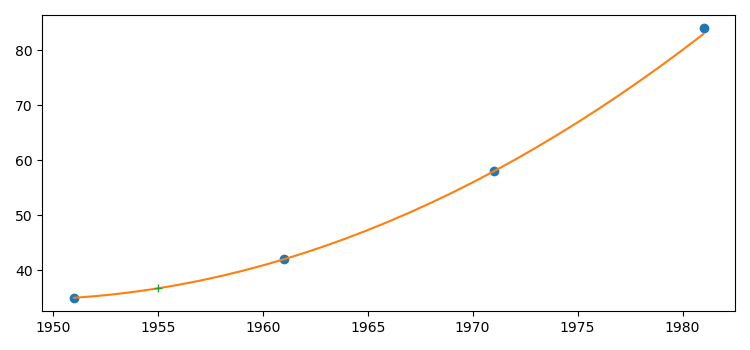
\includegraphics[width=.9\linewidth]{question1_a.png}
\end{center}
\section{Question 2}
\label{sec:org7dc9725}
Show that given a linear function i.e \(y = ax+b\) . You'll need at most 1 iteration of newton-rhapson to find the root
\subsection{Solution}
\label{sec:org68fd458}
Let \(x\in \mathbb{R}\) if \(x = \frac{-b}{a}\) we are done

else , let \(x\not = \frac{-b}{a}\) run 1 iteration of newton-rhapson and show that \(x_1=\frac{-b}{a}\)

\[ x_1 = x - \frac{y(x)}{y'(x)} \]
\[ x_1 = x - \frac{ax+b}{a} \]
\[ x_1 = x - x +\frac{-b}{a} \]
\[ x_1 = \frac{-b}{a} \]
\qedsymbol{}

\newpage
\section{Question 3}
\label{sec:orgaaddb0e}
Given the function \(f\) and let \(Q(x)\) be the interpolation of \(f\) at

\((x_0,x_1 , ... , x_n)\)

and let \(P(x)\) be the newton interpolation of points
\((x_0,x_1 , ... , x_n , t ,t )\)
for arbitrary \(t \in \mathbb{R}\)

Writing \(Q(x)\) explicitly we'll have
\begin{align}
Q(x) = [y_0] + [y_0,y_1](x-x_0) + \cdots + [y_0,\ldots,y_n](x-x_0)(x-x_1)\cdots(x-x_{n-1})
\end{align}

and writing \(P(x)\) explicitly grants us
\begin{align*}
P(x) &= [y_0] + [y_0,y_1](x-x_0) + \cdots + [y_0,\ldots,y_n](x-x_0)(x-x_1)\cdots(x-x_{n-1})+ \\
& [y_0,\ldots,y_n , t](x-x_0)(x-x_1)\cdots(x-x_{n-1})(x-t) + \\
& [y_0,\ldots,y_n,t,t](x-x_0)(x-x_1)\cdots(x-x_{n-1})(x-t)^2 \\
\end{align*}

Clearly we can see that

\begin{align*}
P(x) - Q(x)  =
& [y_0,\ldots,y_n , t](x-x_0)(x-x_1)\cdots(x-x_{n-1})(x-t) + \\
& [y_0,\ldots,y_n,t,t](x-x_0)(x-x_1)\cdots(x-x_{n-1})(x-t)^2 \\
\end{align*}



\newpage
\section{Question 4}
\label{sec:org14358a2}
Evaluate the integral
\[ \int _{0}^{1}\frac{1}{1+x^{3}} dx \]
using the trapezoidal rule we have the following formula

\[ \int_{a}^{b} f(x)dx = \frac{b-a}{n}\big( \frac{f(a)+f(b)}{2} + \sum_{i=1}^{n-1}f(a+\frac{b-a}{n}i) \big) \]

Using python code we have
\begin{Code}
\begin{Verbatim}
\color{EFD}\EFk{def} \EFf{f}(x):
    \EFk{return} \EFhn{1}/(\EFhn{1}+x**\EFhn{3})
\EFv{a} = \EFhn{0} ; \EFv{b} = \EFhn{1} ; \EFv{n} =\EFhn{4}
\EFk{return} (b - a )/n *( (f(b)-f(a))/\EFhn{2} + \EFb{sum}([f(a+(b-a)*i/n) \EFk{for} i \EFk{in} \EFb{range}(\EFhn{1},n-\EFhn{1}) ]) )

\end{Verbatim}
\end{Code}

\begin{verbatim}
0.4058760683760684
\end{verbatim}


\begin{Code}
\begin{Verbatim}
\color{EFD}\EFk{def} \EFf{f}(x):
    \EFk{return} \EFhn{1}/(\EFhn{1}+x**\EFhn{3})
\EFv{a} = \EFhn{0} ; \EFv{b} = \EFhn{1} ; \EFv{n} =\EFhn{40}
\EFk{return} (b - a )/n *( (f(b)-f(a))/\EFhn{2} + \EFb{sum}([f(a+(b-a)*i/n) \EFk{for} i \EFk{in} \EFb{range}(\EFhn{1},n-\EFhn{1}) ]) )

\end{Verbatim}
\end{Code}

\begin{verbatim}
0.7976353006745376
\end{verbatim}


Happily we can see that after 40 iteration we are really close to the true solution which is 0.83525
\[ relative error = \frac{\Delta y}{y} = \frac{0.83525 - 0.7976353006745376}{0.83525}= 0.045 \]


\newpage
\section{Question 5}
\label{sec:org77fab99}
Write a program in C++ that can calculate the integral from 0 to 1 divided by n seqments

\begin{Code}
\begin{Verbatim}
\color{EFD}\EFpp{\#include} \textcolor[HTML]{707183}{<}\EFs{iostream}\textcolor[HTML]{707183}{>}
\EFt{double} \EFf{f}\EFrda{(}\EFt{double} \EFv{x}\EFrda{)}\EFrda{\{} \EFcd{//} \EFc{Example function , one can pick anyfunction he wants}
    \EFk{return} \EFhn{1}/\EFrdb{(}x*x*x + \EFhn{1}\EFrdb{)};
\EFrda{\}}
\EFt{double} \EFf{integral\_calculator}\EFrda{(}\EFt{int} \EFv{n} , \EFt{double} \EFv{a} = \EFhn{0} , \EFt{double} \EFv{b}=\EFhn{1}\EFrda{)}\EFrda{\{}
    \EFt{double} \EFv{my\_sum} = \EFhn{0};
   \EFk{for}\EFrdb{(}\EFt{int} \EFv{i} =\EFhn{1}; i < n-\EFhn{1}; i++\EFrdb{)}\EFrdb{\{}
       my\_sum += f\EFrdc{(}a+\EFrdd{(}b-a\EFrdd{)}*i/n\EFrdc{)};
   \EFrdb{\}}
    \EFk{return} \EFrdb{(}b-a\EFrdb{)}/n*\EFrdb{(}\EFrdc{(}f\EFrdd{(}b\EFrdd{)}+f\EFrdd{(}a\EFrdd{)}\EFrdc{)}/\EFhn{2} + my\_sum\EFrdb{)};
\EFrda{\}}
\EFt{int} \EFf{main}\EFrda{(}\EFrda{)} \EFrda{\{}
    \EFo{std}::cout << \EFs{"The answer is :"} << integral\_calculator\EFrdb{(}\EFhn{19}\EFrdb{)};
    \EFk{return} \EFhn{0};
\EFrda{\}}

\end{Verbatim}
\end{Code}

\begin{verbatim}
The answer is :0.80703
\end{verbatim}
\section{Question 6}
\label{sec:org822426f}
Write a Program in C++ that given n+1 point on \(\mathbb{R}^2\) Creates interpolation polinom
\newpage
\subsection{Answer a - lagrange interpolation}
\label{sec:org530242f}
Here is code snippet that implement lagrange interpolation
\begin{Code}
\begin{Verbatim}
\color{EFD}\EFpp{\#include} \textcolor[HTML]{707183}{<}\EFs{iostream}\textcolor[HTML]{707183}{>}
\EFpp{\#include} \textcolor[HTML]{707183}{<}\EFs{vector}\textcolor[HTML]{707183}{>}
\EFpp{\#include} \textcolor[HTML]{707183}{<}\EFs{tuple}\textcolor[HTML]{707183}{>}
\EFpp{\#include} \textcolor[HTML]{707183}{<}\EFs{utility}\textcolor[HTML]{707183}{>}
\EFk{using} \EFk{namespace} \EFo{std};
\EFt{double} \EFf{lagrange\_basis}\EFrda{(}\EFt{double} \EFv{x},\EFt{int} \EFv{j},\EFt{vector}\EFrdb{<}\EFt{tuple}\EFrdc{<}\EFt{double},\EFt{double}\EFrdc{>}    \EFrdb{>} \EFv{data} \EFrda{)}\EFrda{\{}
    \EFt{double} \EFv{p} = \EFhn{1};
    \EFk{auto} \EFrdb{[}x\_j,y\_j\EFrdb{]} = data\EFrdb{[}j\EFrdb{]};
    data.erase\EFrdb{(}data.begin\EFrdc{(}\EFrdc{)}+j\EFrdb{)};
        \EFk{for}\EFrdb{(}\EFk{auto} \EFrdc{[}x\_i,y\_i\EFrdc{]} : data\EFrdb{)}\EFrdb{\{}
            p *= \EFrdc{(}x-x\_i\EFrdc{)}/\EFrdc{(}x\_j-x\_i\EFrdc{)};
    \EFrdb{\}}
    data.insert\EFrdb{(}data.begin\EFrdc{(}\EFrdc{)}+j,make\_tuple\EFrdc{(}x\_j,y\_j\EFrdc{)}\EFrdb{)};
    \EFk{return} p;
\EFrda{\}}
\EFt{double} \EFf{lagrange\_interpolation}\EFrda{(}\EFt{double} \EFv{x} ,\EFt{vector}\EFrdb{<}\EFt{tuple}\EFrdc{<}\EFt{double},\EFt{double}\EFrdc{>}    \EFrdb{>} \EFv{data}\EFrda{)}\EFrda{\{}
    \EFt{double} \EFv{sum\_lagrange} = \EFhn{0};
    \EFt{int} \EFv{j} = \EFhn{0};
    \EFk{for}\EFrdb{(}\EFk{auto} \EFrdc{[}x\_i,y\_i\EFrdc{]} :data\EFrdb{)}\EFrdb{\{}
        sum\_lagrange += y\_i*lagrange\_basis\EFrdc{(}x,j,data\EFrdc{)};
        j++;
    \EFrdb{\}}
    \EFk{return} sum\_lagrange;
\EFrda{\}}
\EFt{int} \EFf{main}\EFrda{(}\EFrda{)}\EFrda{\{}
    \EFt{vector}\EFrdb{<}\EFt{tuple}\EFrdc{<}\EFt{double},\EFt{double}\EFrdc{>}    \EFrdb{>} \EFv{data} ;
    data.push\_back\EFrdb{(}make\_tuple\EFrdc{(}\EFhn{1},\EFhn{2}\EFrdc{)}\EFrdb{)};
    data.push\_back\EFrdb{(}make\_tuple\EFrdc{(}\EFhn{3},\EFhn{4}\EFrdc{)}\EFrdb{)};

      \EFcd{//}\EFc{lagrange\_basis(30,0,data);}
        cout << \EFs{"Given the x = 2 the interpolation is "} <<lagrange\_interpolation\EFrdb{(}\EFhn{2},data\EFrdb{)};
\EFrda{\}}
\end{Verbatim}
\end{Code}

\begin{verbatim}
Given the x = 2 the interpolation is 3
\end{verbatim}


But It makes sense that the point (2,3) is on the interpolation of the data (1,2) , (3,4)
because it's a simple line !
\subsection{Answer B - Use Newton Interpolation}
\label{sec:org0abc4cc}
Implement via the programming language c++ the newton interpolation

\begin{Code}
\begin{Verbatim}
\color{EFD}\EFcd{//} \EFc{Calculate the finite difference function}
\EFpp{\#include} \textcolor[HTML]{707183}{<}\EFs{iostream}\textcolor[HTML]{707183}{>}
\EFpp{\#include} \textcolor[HTML]{707183}{<}\EFs{vector}\textcolor[HTML]{707183}{>}
\EFk{using} \EFk{namespace} \EFo{std};
\EFt{double} \EFf{div\_diff}\EFrda{(}\EFt{vector}\EFrdb{<}\EFt{double}\EFrdb{>}\EFv{x}, \EFt{vector}\EFrdb{<}\EFt{double}\EFrdb{>}\EFv{y}\EFrda{)}\EFrda{\{}
    \EFk{if} \EFrdb{(}x.size\EFrdc{(}\EFrdc{)} == \EFhn{1}\EFrdb{)}
        \EFk{return} y\EFrdb{[}\EFhn{0}\EFrdb{]};
    \EFo{vector}\EFrdb{<}\EFt{double}\EFrdb{>}::\EFt{const\_iterator} \EFv{start} = x.begin\EFrdb{(}\EFrdb{)} + \EFhn{1};
    \EFo{vector}\EFrdb{<}\EFt{double}\EFrdb{>}::\EFt{const\_iterator} \EFv{end}  = x.end\EFrdb{(}\EFrdb{)};
    \EFt{vector}\EFrdb{<}\EFt{double}\EFrdb{>} \EFv{x\_from\_1}\EFrdb{(}start, end\EFrdb{)};
    start = y.begin\EFrdb{(}\EFrdb{)} +\EFhn{1};
    end = y.end\EFrdb{(}\EFrdb{)};
    \EFt{vector}\EFrdb{<}\EFt{double}\EFrdb{>} \EFv{y\_from\_1}\EFrdb{(}start, end\EFrdb{)};
    start = x.begin\EFrdb{(}\EFrdb{)};
    end = x.end\EFrdb{(}\EFrdb{)} - \EFhn{1};
    \EFt{vector}\EFrdb{<}\EFt{double}\EFrdb{>} \EFv{x\_no\_last\_element}\EFrdb{(}start, end\EFrdb{)};
    start = y.begin\EFrdb{(}\EFrdb{)};
    end = y.end\EFrdb{(}\EFrdb{)} - \EFhn{1};
    \EFt{vector}\EFrdb{<}\EFt{double}\EFrdb{>} \EFv{y\_no\_last\_element}\EFrdb{(}start, end\EFrdb{)};
    \EFk{return} \EFrdb{(}\EFrdc{(}div\_diff\EFrdd{(}x\_from\_1 , y\_from\_1\EFrdd{)} - div\_diff\EFrdd{(}x\_no\_last\_element,y\_no\_last\_element\EFrdd{)}\EFrdc{)}\EFrdb{)}/\EFrdb{(}x.back\EFrdc{(}\EFrdc{)} - x.front\EFrdc{(}\EFrdc{)}\EFrdb{)};
    \EFrda{\}}
\EFt{int} \EFf{main}\EFrda{(}\EFrda{)}\EFrda{\{}
    \EFcd{//} \EFc{example of usage}
    \EFt{vector} \EFrdb{<}\EFt{double}\EFrdb{>} \EFv{x} = \EFrdb{\{}\EFhn{8.1} , \EFhn{8.3}\EFrdb{\}};
    \EFt{vector} \EFrdb{<}\EFt{double}\EFrdb{>} \EFv{y} = \EFrdb{\{}\EFhn{16.9446} , \EFhn{17.56492}\EFrdb{\}};

    \EFo{std}::cout << \EFs{"The div different is "} << div\_diff\EFrdb{(}x,y\EFrdb{)};
    \EFk{return} \EFhn{1};
\EFrda{\}}
\end{Verbatim}
\end{Code}

\begin{verbatim}
The div different is 3.1016
\end{verbatim}


\begin{Code}
\begin{Verbatim}
\color{EFD}\EFk{def} \EFf{div\_diff}(x , y):
    \EFk{if} \EFb{len}(x) == \EFhn{1}:
        \EFk{return} y[\EFhn{0}]
    \EFk{return} (div\_diff(x[\EFhn{1}:],y[\EFhn{1}:]) - div\_diff(x[:-\EFhn{1}],y[:-\EFhn{1}]))/(x[-\EFhn{1}] - x[\EFhn{0}])
\EFcd{\#}\EFc{example}
\EFk{return} div\_diff([\EFhn{8.1},\EFhn{8.3}],[\EFhn{16.9446} , \EFhn{17.56492}])
\end{Verbatim}
\end{Code}

\begin{verbatim}
3.1015999999999813
\end{verbatim}


Clearly in python it's more elegant
In order to calculate the the final newton interpolation I'll use the same code from question just in c++

\begin{Code}
\begin{Verbatim}
\color{EFD}\EFpp{\#include} \textcolor[HTML]{707183}{<}\EFs{vector}\textcolor[HTML]{707183}{>}
\EFpp{\#include} \textcolor[HTML]{707183}{<}\EFs{iostream}\textcolor[HTML]{707183}{>}
\EFpp{\#include} \textcolor[HTML]{707183}{<}\EFs{cmath}\textcolor[HTML]{707183}{>}
\EFk{using} \EFk{namespace} \EFo{std};
\EFt{double} \EFf{newton\_interpolation}\EFrda{(}\EFt{double} \EFv{x} ,\EFt{vector}\EFrdb{<}\EFt{double}\EFrdb{>} \EFv{x\_arr} , \EFt{vector}\EFrdb{<}\EFt{double}\EFrdb{>}\EFv{div\_diff\_arr}\EFrda{)}\EFrda{\{}
  \EFt{double} \EFv{acc} = \EFhn{0};
  \EFk{for} \EFrdb{(}\EFt{int} \EFv{i} =\EFhn{0};i < div\_diff\_arr.size\EFrdc{(}\EFrdc{)} ;i++\EFrdb{)}\EFrdb{\{}
      \EFt{double} \EFv{mal} = div\_diff\_arr\EFrdc{[}i\EFrdc{]};
      \EFk{for}\EFrdc{(}\EFt{int} \EFv{j} =\EFhn{0} ; j < i ; j++\EFrdc{)}\EFrdc{\{}
          mal *=  \EFo{std}::pow\EFrdd{(}\EFrda{(}x-x\_arr\EFrdb{[}j\EFrdb{]}\EFrda{)},j\EFrdd{)} ;
        \EFrdc{\}}
          acc += mal;
\EFrdb{\}}
  \EFk{return} acc;
\EFrda{\}}
\EFt{int} \EFf{main}\EFrda{(}\EFrda{)}\EFrda{\{}
    \EFt{vector} \EFrdb{<}\EFt{double} \EFrdb{>} \EFv{x} = \EFrdb{\{}\EFhn{1951} , \EFhn{1961} , \EFhn{1971} , \EFhn{1981}\EFrdb{\}}; \EFcd{//} \EFc{from question 1}
    \EFt{vector} \EFrdb{<}\EFt{double} \EFrdb{>} \EFv{div\_diff\_arr} = \EFrdb{\{}\EFhn{35} , \EFhn{0.7} , \EFhn{0.045}\EFrdb{\}}; \EFcd{//} \EFc{from question 1}
    \EFo{std}::cout << \EFs{"Interpolatoin is "} << newton\_interpolation\EFrdb{(}\EFhn{1955} , x , div\_diff\_arr\EFrdb{)};
\EFrda{\}}


\end{Verbatim}
\end{Code}

\begin{verbatim}
Interpolatoin is 35.43
\end{verbatim}


Please note that the result 35.43 is close to 36.72 , now I'll combine the 2 function together to have entire pipe


The following code looks the same but it combines both of the functions

\begin{Code}
\begin{Verbatim}
\color{EFD}\EFpp{\#include} \textcolor[HTML]{707183}{<}\EFs{vector}\textcolor[HTML]{707183}{>}
\EFpp{\#include} \textcolor[HTML]{707183}{<}\EFs{iostream}\textcolor[HTML]{707183}{>}
\EFpp{\#include} \textcolor[HTML]{707183}{<}\EFs{cmath}\textcolor[HTML]{707183}{>}
\EFk{using} \EFk{namespace} \EFo{std};

\EFt{double} \EFf{div\_diff}\EFrda{(}\EFt{vector}\EFrdb{<}\EFt{double}\EFrdb{>}\EFv{x}, \EFt{vector}\EFrdb{<}\EFt{double}\EFrdb{>}\EFv{y}\EFrda{)}\EFrda{\{}
    \EFk{if} \EFrdb{(}x.size\EFrdc{(}\EFrdc{)} == \EFhn{1}\EFrdb{)}
        \EFk{return} y\EFrdb{[}\EFhn{0}\EFrdb{]};
    \EFo{vector}\EFrdb{<}\EFt{double}\EFrdb{>}::\EFt{const\_iterator} \EFv{start} = x.begin\EFrdb{(}\EFrdb{)} + \EFhn{1};
    \EFo{vector}\EFrdb{<}\EFt{double}\EFrdb{>}::\EFt{const\_iterator} \EFv{end}  = x.end\EFrdb{(}\EFrdb{)};
    \EFt{vector}\EFrdb{<}\EFt{double}\EFrdb{>} \EFv{x\_from\_1}\EFrdb{(}start, end\EFrdb{)};
    start = y.begin\EFrdb{(}\EFrdb{)} +\EFhn{1};
    end = y.end\EFrdb{(}\EFrdb{)};
    \EFt{vector}\EFrdb{<}\EFt{double}\EFrdb{>} \EFv{y\_from\_1}\EFrdb{(}start, end\EFrdb{)};
    start = x.begin\EFrdb{(}\EFrdb{)};
    end = x.end\EFrdb{(}\EFrdb{)} - \EFhn{1};
    \EFt{vector}\EFrdb{<}\EFt{double}\EFrdb{>} \EFv{x\_no\_last\_element}\EFrdb{(}start, end\EFrdb{)};
    start = y.begin\EFrdb{(}\EFrdb{)};
    end = y.end\EFrdb{(}\EFrdb{)} - \EFhn{1};
    \EFt{vector}\EFrdb{<}\EFt{double}\EFrdb{>} \EFv{y\_no\_last\_element}\EFrdb{(}start, end\EFrdb{)};
    \EFk{return} \EFrdb{(}\EFrdc{(}div\_diff\EFrdd{(}x\_from\_1 , y\_from\_1\EFrdd{)} - div\_diff\EFrdd{(}x\_no\_last\_element,y\_no\_last\_element\EFrdd{)}\EFrdc{)}\EFrdb{)}/\EFrdb{(}x.back\EFrdc{(}\EFrdc{)} - x.front\EFrdc{(}\EFrdc{)}\EFrdb{)};
    \EFrda{\}}

\EFt{double} \EFf{newton\_interpolation}\EFrda{(}\EFt{double} \EFv{x} ,\EFt{vector}\EFrdb{<}\EFt{double}\EFrdb{>} \EFv{x\_arr} , \EFt{vector}\EFrdb{<}\EFt{double}\EFrdb{>}\EFv{div\_diff\_arr}\EFrda{)}\EFrda{\{}
  \EFt{double} \EFv{acc} = \EFhn{0};
  \EFk{for} \EFrdb{(}\EFt{int} \EFv{i} =\EFhn{0};i < div\_diff\_arr.size\EFrdc{(}\EFrdc{)} ;i++\EFrdb{)}\EFrdb{\{}
      \EFt{double} \EFv{mal} = div\_diff\_arr\EFrdc{[}i\EFrdc{]};
      \EFk{for}\EFrdc{(}\EFt{int} \EFv{j} =\EFhn{0} ; j < i ; j++\EFrdc{)}\EFrdc{\{}
          mal *=  \EFo{std}::pow\EFrdd{(}\EFrda{(}x-x\_arr\EFrdb{[}j\EFrdb{]}\EFrda{)},j\EFrdd{)} ;
        \EFrdc{\}}
          acc += mal;
\EFrdb{\}}
  \EFk{return} acc;
\EFrda{\}}
\EFt{vector} \EFrda{<}\EFt{double}\EFrda{>} \EFf{subarray}\EFrda{(}\EFt{vector} \EFrdb{<}\EFt{double}\EFrdb{>} \EFv{arr} , \EFk{auto} \EFv{first} , \EFk{auto} \EFv{last} \EFrda{)}\EFrda{\{}
    \EFt{vector}\EFrdb{<}\EFt{double}\EFrdb{>} \EFv{subarr}\EFrdb{(}first , last\EFrdb{)};
    \EFk{return} subarr;
\EFrda{\}}
\EFt{int} \EFf{main}\EFrda{(}\EFrda{)}\EFrda{\{}
    \EFt{vector} \EFrdb{<}\EFt{double} \EFrdb{>} \EFv{x} = \EFrdb{\{}\EFhn{1951} , \EFhn{1961} , \EFhn{1971} , \EFhn{1981}\EFrdb{\}}; \EFcd{//} \EFc{from question 1}
    \EFt{vector} \EFrdb{<}\EFt{double} \EFrdb{>} \EFv{y} = \EFrdb{\{}\EFhn{35},\EFhn{42},\EFhn{58},\EFhn{84}\EFrdb{\}}; \EFcd{//} \EFc{from question 1}
    \EFt{vector} \EFrdb{<}\EFt{double}\EFrdb{>} \EFv{div\_diff\_arr};
    \EFt{vector} \EFrdb{<}\EFt{double}\EFrdb{>}\EFv{sub\_x};
    \EFt{vector} \EFrdb{<}\EFt{double}\EFrdb{>} \EFv{sub\_y};
    \EFk{auto} \EFv{first\_x} = x.begin\EFrdb{(}\EFrdb{)};
    \EFk{auto} \EFv{last\_x} = x.begin\EFrdb{(}\EFrdb{)};
    \EFk{auto} \EFv{first\_y} = y.begin\EFrdb{(}\EFrdb{)};
    \EFk{auto} \EFv{last\_y} = y.begin\EFrdb{(}\EFrdb{)};
    \EFk{for}\EFrdb{(} \EFt{int} \EFv{i} =\EFhn{0} ; i < x.size\EFrdc{(}\EFrdc{)} ; i++ \EFrdb{)}\EFrdb{\{}
           first\_x = x.begin\EFrdc{(}\EFrdc{)};
           last\_x = x.begin\EFrdc{(}\EFrdc{)} + i + \EFhn{1};
           sub\_x = subarray\EFrdc{(}x, first\_x, last\_x\EFrdc{)};
           first\_y = y.begin\EFrdc{(}\EFrdc{)};
           last\_y = y.begin\EFrdc{(}\EFrdc{)} + i + \EFhn{1};
           sub\_y = subarray\EFrdc{(}y,first\_y, last\_y\EFrdc{)};
        div\_diff\_arr.push\_back\EFrdc{(}div\_diff\EFrdd{(}sub\_x , sub\_y   \EFrdd{)}\EFrdc{)};
    \EFrdb{\}}
    \EFo{std}::cout << \EFs{"Interpolatoin is "} << newton\_interpolation\EFrdb{(}\EFhn{1955} , x , div\_diff\_arr\EFrdb{)};
\EFrda{\}}


\end{Verbatim}
\end{Code}

\begin{verbatim}
Interpolatoin is 35.174
\end{verbatim}

\newpage
\section{Question 7}
\label{sec:org81ccd41}
Calculate the newton interpolation polinom of the function
\[ f(x) = x^3 \]

using the the set of point
\[ (1,1),(2,8),(3,27),(4,64)  \]

using the function from question the

\begin{table}[htbp]
\label{data_question7}
\centering
\begin{tabular}{lrrrrr}
\hline
x & 1 & 2 & 3 & 4 & 5\\
\hline
y & 1 & 8 & 27 & 64 & 125\\
\hline
\end{tabular}
\end{table}

I'll calculate the coefficient
\[ [y_0] , [y_0 , y_1] , [y_0 , y_1,y_2] , [y_0 , y_1 , y_2 , y_3]  \]


\begin{Code}
\begin{Verbatim}
\color{EFD}\EFk{def} \EFf{div\_diff}(x , y):
    \EFk{if} \EFb{len}(x) == \EFhn{1}:
        \EFk{return} y[\EFhn{0}]
    \EFk{return} (div\_diff(x[\EFhn{1}:],y[\EFhn{1}:]) - div\_diff(x[:-\EFhn{1}],y[:-\EFhn{1}]))/(x[-\EFhn{1}] - x[\EFhn{0}])
\EFcd{\#}\EFc{example}
\EFcd{\#}\EFc{return div\_diff([8.1,8.3],[16.9446 , 17.56492])}
\EFv{x} = my\_data[\EFhn{0}][\EFhn{1}:] \EFcd{\#}\EFc{Get the data from the table}
\EFv{y} = my\_data[\EFhn{1}][\EFhn{1}:] \EFcd{\#} \EFc{Get the data from the table}
\EFv{newton\_coeff} = [div\_diff(x[:i], y[:i]) \EFk{for} i \EFk{in} \EFb{range}(\EFhn{1},\EFb{len}(x))]
\EFk{return} newton\_coeff
\end{Verbatim}
\end{Code}

\begin{center}
\begin{tabular}{rrrr}
1 & 7.0 & 6.0 & 1.0\\
\end{tabular}
\end{center}

which is exactly
\begin{center}
\begin{tabular}{rrrr}
\hline
{[}y\textsubscript{0}] & {[}y\textsubscript{0} , y\textsubscript{1} ] & {[}y\textsubscript{0} , y\textsubscript{1} , y\textsubscript{2} ] & {[}y\textsubscript{0} , y\textsubscript{1} ,y\textsubscript{2} ,y\textsubscript{3} ]\\
1 & 7.0 & 6.0 & 1.0\\
\hline
\end{tabular}
\end{center}


From the formula of newton interpolation

\begin{align}
N(x) = [y_0] + [y_0,y_1](x-x_0) + \cdots + [y_0,\ldots,y_k](x-x_0)(x-x_1)\cdots(x-x_{k-1})
\end{align}


\begin{equation}
N(x) = 1+7(x-1)+6(x-1)(x-2) + 1(x-1)(x-2)(x-3)
\end{equation}


\begin{Code}
\begin{Verbatim}
\color{EFD}\EFk{from} sympy \EFk{import} symbols , init\_printing , simplify
\EFv{x} = symbols(\EFs{'x'})
init\_printing(use\_unicode=\EFo{True})
\EFk{return} simplify(\EFhn{1}+\EFhn{7}*(x-\EFhn{1})+\EFhn{6}*(x-\EFhn{1})*(x-\EFhn{2}) + \EFhn{1}*(x-\EFhn{1})*(x-\EFhn{2})*(x-\EFhn{3}))
\end{Verbatim}
\end{Code}

\begin{verbatim}
x**3
\end{verbatim}



Which means that our interpolation simplify to \(x^3\)


Note that the error from the function \(f(x)  = x^3\) is
\[ E = |f(x) - N(x)| = |x^3- x^3| = 0  \]
which means that for all \(x \in \mathbb{R}\)  the error is 0
\end{document}
